\documentclass{beamer}
\usepackage[english]{babel}
\usepackage{tikz}
\usetikzlibrary{calc}

\setbeamertemplate{navigation symbols}{}

\title[PL3GA Visualisation]{Visualising objects in the geometric algebra of projective line geometry}
\author{Patrick de Kok}
\institute{Universiteit van Amsterdam}

\newcommand{\Rl}{\ensuremath{\mathbb{R}^{3,3}}}
\newcommand{\V}[1]{\ensuremath{\mathbf{#1}}}

\begin{document}
\begin{frame}
\titlepage
\end{frame}

\begin{frame}{Approach}
\begin{enumerate}
\item Explore representation space
\item Computing geometric interpretation
\item Implement drawing routines
\end{enumerate}
\end{frame}

\begin{frame}{Explore representation space}
\begin{itemize}%[<+->]
\item Pl\"ucker coordinates: 3D lines are 6D null vectors 
\begin{itemize}
\item Representation is homogeneous
\end{itemize}
\item Outer product $\wedge$ to generate subspaces
\end{itemize}
Which geometric objects are in the representation space?

\only<1>{
\begin{figure}[b]
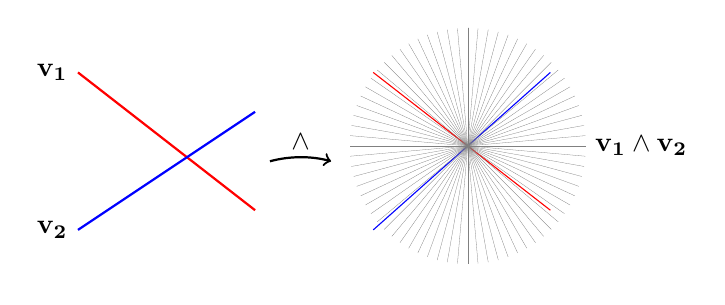
\begin{tikzpicture}
\coordinate (O) at (0,0);
\coordinate (A1) at (-0.75, 1);
\coordinate (A2) at (1.5, -0.75);
\coordinate (B1) at (-0.75, -1);
\coordinate (B2) at (1.5, 0.5);
\coordinate (D1) at (3, 1);
\coordinate (D2) at (5.25, -0.75);
\coordinate (E1) at (3, -1);
\coordinate (E2) at (5.25, 1);

\draw[thick, red] (A1) node[left,black] {$\V{v_1}$} -- (A2);
\draw[thick, blue] (B1) node[left,black] {$\V{v_2}$} -- (B2);

\draw[red] (D1) -- (D2);
\draw[blue] (E1) -- (E2);
\coordinate (C) at (intersection cs: first line={(D1) -- (D2)}, second line={(E1)--(E2)});

\coordinate (M) at (intersection cs: first line={(A2)--(D1)}, second line={(B2)--(E1)});
\draw[thick, ->] (M) ++(0,-1.5) ++(105:1.5) arc (105:75:1.5);
\draw (M) +(0,0.2) node {$\wedge$};

\draw[ultra thin, gray] (C) -- +(0:1.5) node[right,black] {$\V{v_1} \wedge \V{v_2}$} -- +(0:-1.5);
\draw[ultra thin, gray] (C) -- +(5:1.5) -- +(5:-1.5);
\draw[ultra thin, gray] (C) -- +(10:1.5) -- +(10:-1.5);
\draw[ultra thin, gray] (C) -- +(15:1.5) -- +(15:-1.5);
\draw[ultra thin, gray] (C) -- +(20:1.5) -- +(20:-1.5);
\draw[ultra thin, gray] (C) -- +(25:1.5) -- +(25:-1.5);
\draw[ultra thin, gray] (C) -- +(30:1.5) -- +(30:-1.5);
\draw[ultra thin, gray] (C) -- +(35:1.5) -- +(35:-1.5);
\draw[ultra thin, gray] (C) -- +(40:1.5) -- +(40:-1.5);
\draw[ultra thin, gray] (C) -- +(45:1.5) -- +(45:-1.5);
\draw[ultra thin, gray] (C) -- +(50:1.5) -- +(50:-1.5);
\draw[ultra thin, gray] (C) -- +(55:1.5) -- +(55:-1.5);
\draw[ultra thin, gray] (C) -- +(60:1.5) -- +(60:-1.5);
\draw[ultra thin, gray] (C) -- +(65:1.5) -- +(65:-1.5);
\draw[ultra thin, gray] (C) -- +(70:1.5) -- +(70:-1.5);
\draw[ultra thin, gray] (C) -- +(75:1.5) -- +(75:-1.5);
\draw[ultra thin, gray] (C) -- +(80:1.5) -- +(80:-1.5);
\draw[ultra thin, gray] (C) -- +(85:1.5) -- +(85:-1.5);
\draw[ultra thin, gray] (C) -- +(90:1.5) -- +(90:-1.5);
\draw[ultra thin, gray] (C) -- +(95:1.5) -- +(95:-1.5);
\draw[ultra thin, gray] (C) -- +(100:1.5) -- +(100:-1.5);
\draw[ultra thin, gray] (C) -- +(105:1.5) -- +(105:-1.5);
\draw[ultra thin, gray] (C) -- +(110:1.5) -- +(110:-1.5);
\draw[ultra thin, gray] (C) -- +(115:1.5) -- +(115:-1.5);
\draw[ultra thin, gray] (C) -- +(120:1.5) -- +(120:-1.5);
\draw[ultra thin, gray] (C) -- +(125:1.5) -- +(125:-1.5);
\draw[ultra thin, gray] (C) -- +(130:1.5) -- +(130:-1.5);
\draw[ultra thin, gray] (C) -- +(135:1.5) -- +(135:-1.5);
\draw[ultra thin, gray] (C) -- +(140:1.5) -- +(140:-1.5);
\draw[ultra thin, gray] (C) -- +(145:1.5) -- +(145:-1.5);
\draw[ultra thin, gray] (C) -- +(150:1.5) -- +(150:-1.5);
\draw[ultra thin, gray] (C) -- +(155:1.5) -- +(155:-1.5);
\draw[ultra thin, gray] (C) -- +(160:1.5) -- +(160:-1.5);
\draw[ultra thin, gray] (C) -- +(165:1.5) -- +(165:-1.5);
\draw[ultra thin, gray] (C) -- +(170:1.5) -- +(170:-1.5);
\draw[ultra thin, gray] (C) -- +(175:1.5) -- +(175:-1.5);
\end{tikzpicture}
\end{figure}
}
\only<2>{
\begin{figure}[b]
\begin{tikzpicture}
\coordinate (O) at (0,0);
\coordinate (x1) at (-0.75, 0.3);
\coordinate (x2) at (1.5, 0.0);
\coordinate (y1) at (-0.55, -0.55);
\coordinate (y2) at (1.5, -0.10);
\coordinate (D1) at ($(x1)+(3.75, 0)$);
\coordinate (D2) at ($(x2)+(3.75, 0)$);
\coordinate (E1) at ($(y1)+(3.75, 0)$);
\coordinate (E2) at ($(y2)+(3.75, 0)$);

\draw[thick, red] (A1) node[left,black] {$\V{v_1}$} -- (A2);
\draw[thick, blue] (B1) node[left,black] {$\V{v_2}$} -- (B2);

\draw ($(D2)!0.5!(E2)$) ++(1,0) node {$\V{v_1} \wedge \V{v_2}$};

\coordinate (M) at (intersection cs: first line={(A2)--(D1)}, second line={(B2)--(E1)});
\draw[thick, ->] ($(A2)!0.5!(D1)$) ++(0,-1.5) ++(105:1.5) arc (105:75:1.5);
\draw ($(A2)!0.5!(D1)$) +(0,0.2) node {$\wedge$};

\draw[ultra thin, gray] ($(D1)!0.0!(D2)$) -- ($(E1)!0.0!(E2)$);
\draw[ultra thin, gray] ($(D1)!0.0!(D2)$) -- ($(E1)!0.2!(E2)$);
\draw[ultra thin, gray] ($(D1)!0.0!(D2)$) -- ($(E1)!0.4!(E2)$);
\draw[ultra thin, gray] ($(D1)!0.0!(D2)$) -- ($(E1)!0.6!(E2)$);
\draw[ultra thin, gray] ($(D1)!0.0!(D2)$) -- ($(E1)!0.8!(E2)$);
\draw[ultra thin, gray] ($(D1)!0.0!(D2)$) -- ($(E1)!1.0!(E2)$);
\draw[ultra thin, gray] ($(D1)!0.2!(D2)$) -- ($(E1)!0.0!(E2)$);
\draw[ultra thin, gray] ($(D1)!0.2!(D2)$) -- ($(E1)!0.2!(E2)$);
\draw[ultra thin, gray] ($(D1)!0.2!(D2)$) -- ($(E1)!0.4!(E2)$);
\draw[ultra thin, gray] ($(D1)!0.2!(D2)$) -- ($(E1)!0.6!(E2)$);
\draw[ultra thin, gray] ($(D1)!0.2!(D2)$) -- ($(E1)!0.8!(E2)$);
\draw[ultra thin, gray] ($(D1)!0.2!(D2)$) -- ($(E1)!1.0!(E2)$);
\draw[ultra thin, gray] ($(D1)!0.4!(D2)$) -- ($(E1)!0.0!(E2)$);
\draw[ultra thin, gray] ($(D1)!0.4!(D2)$) -- ($(E1)!0.2!(E2)$);
\draw[ultra thin, gray] ($(D1)!0.4!(D2)$) -- ($(E1)!0.4!(E2)$);
\draw[ultra thin, gray] ($(D1)!0.4!(D2)$) -- ($(E1)!0.6!(E2)$);
\draw[ultra thin, gray] ($(D1)!0.4!(D2)$) -- ($(E1)!0.8!(E2)$);
\draw[ultra thin, gray] ($(D1)!0.4!(D2)$) -- ($(E1)!1.0!(E2)$);
\draw[ultra thin, gray] ($(D1)!0.6!(D2)$) -- ($(E1)!0.0!(E2)$);
\draw[ultra thin, gray] ($(D1)!0.6!(D2)$) -- ($(E1)!0.2!(E2)$);
\draw[ultra thin, gray] ($(D1)!0.6!(D2)$) -- ($(E1)!0.4!(E2)$);
\draw[ultra thin, gray] ($(D1)!0.6!(D2)$) -- ($(E1)!0.6!(E2)$);
\draw[ultra thin, gray] ($(D1)!0.6!(D2)$) -- ($(E1)!0.8!(E2)$);
\draw[ultra thin, gray] ($(D1)!0.6!(D2)$) -- ($(E1)!1.0!(E2)$);
\draw[ultra thin, gray] ($(D1)!0.8!(D2)$) -- ($(E1)!0.0!(E2)$);
\draw[ultra thin, gray] ($(D1)!0.8!(D2)$) -- ($(E1)!0.2!(E2)$);
\draw[ultra thin, gray] ($(D1)!0.8!(D2)$) -- ($(E1)!0.4!(E2)$);
\draw[ultra thin, gray] ($(D1)!0.8!(D2)$) -- ($(E1)!0.6!(E2)$);
\draw[ultra thin, gray] ($(D1)!0.8!(D2)$) -- ($(E1)!0.8!(E2)$);
\draw[ultra thin, gray] ($(D1)!0.8!(D2)$) -- ($(E1)!1.0!(E2)$);
\draw[ultra thin, gray] ($(D1)!1.0!(D2)$) -- ($(E1)!0.0!(E2)$);
\draw[ultra thin, gray] ($(D1)!1.0!(D2)$) -- ($(E1)!0.2!(E2)$);
\draw[ultra thin, gray] ($(D1)!1.0!(D2)$) -- ($(E1)!0.4!(E2)$);
\draw[ultra thin, gray] ($(D1)!1.0!(D2)$) -- ($(E1)!0.6!(E2)$);
\draw[ultra thin, gray] ($(D1)!1.0!(D2)$) -- ($(E1)!0.8!(E2)$);
\draw[ultra thin, gray] ($(D1)!1.0!(D2)$) -- ($(E1)!1.0!(E2)$);

\draw[thick, red] (D1) -- (D2);
\draw[thick, blue] (E1) -- (E2);

\end{tikzpicture}
\end{figure}
}
%\only<2>{
%\begin{figure}[b]
%\begin{tikzpicture}
%\coordinate (O) at (0,0);
%\coordinate (A1) at (-0.75, 0.3);
%\coordinate (A2) at (1.5, 0.3);
%\coordinate (B1) at (-0.75, -0.75);
%\coordinate (B2) at (1.5, -0.75);
%\coordinate (D1) at (3, 0.3);
%\coordinate (D2) at (5.25, 0.3);
%\coordinate (E1) at (3, -0.75);
%\coordinate (E2) at (5.25, -0.75);
%
%\draw[thick, red] (A1) node[left,black] {$\V{v_1}$} -- (A2);
%\draw[thick, blue] (B1) node[left,black] {$\V{v_2}$} -- (B2);
%
%\draw[red] (D1) -- (D2);
%\draw[blue] (E1) -- (E2);
%
%\coordinate (C) at (intersection cs: first line={(D1)--(E2)}, second line={(E1)--(D2)});
%
%\draw (C) ++(2,0) node {$\V{v_1} \wedge \V{v_2}$};
%
%\coordinate (M) at (intersection cs: first line={(A2)--(E1)}, second line={(B2)--(D1)});
%\draw[thick, ->] (M) ++(0,-1.5) ++(105:1.5) arc (105:75:1.5);
%\draw (M) +(0,0.2) node {$\wedge$};
%
%\draw[ultra thin, gray] ($(D1)!-0.4!(E1)$) -- ++(2.25, 0);
%\draw[ultra thin, gray] ($(D1)!-0.3!(E1)$) -- ++(2.25, 0);
%\draw[ultra thin, gray] ($(D1)!-0.2!(E1)$) -- ++(2.25, 0);
%\draw[ultra thin, gray] ($(D1)!-0.1!(E1)$) -- ++(2.25, 0);
%\draw[ultra thin, gray] ($(D1)!0.0!(E1)$) -- ++(2.25, 0);
%\draw[ultra thin, gray] ($(D1)!0.1!(E1)$) -- ++(2.25, 0);
%\draw[ultra thin, gray] ($(D1)!0.2!(E1)$) -- ++(2.25, 0);
%\draw[ultra thin, gray] ($(D1)!0.3!(E1)$) -- ++(2.25, 0);
%\draw[ultra thin, gray] ($(D1)!0.4!(E1)$) -- ++(2.25, 0);
%\draw[ultra thin, gray] ($(D1)!0.5!(E1)$) -- ++(2.25, 0);
%\draw[ultra thin, gray] ($(D1)!0.6!(E1)$) -- ++(2.25, 0);
%\draw[ultra thin, gray] ($(D1)!0.7!(E1)$) -- ++(2.25, 0);
%\draw[ultra thin, gray] ($(D1)!0.8!(E1)$) -- ++(2.25, 0);
%\draw[ultra thin, gray] ($(D1)!0.9!(E1)$) -- ++(2.25, 0);
%\draw[ultra thin, gray] ($(D1)!1.0!(E1)$) -- ++(2.25, 0);
%\draw[ultra thin, gray] ($(D1)!1.1!(E1)$) -- ++(2.25, 0);
%\draw[ultra thin, gray] ($(D1)!1.2!(E1)$) -- ++(2.25, 0);
%\draw[ultra thin, gray] ($(D1)!1.3!(E1)$) -- ++(2.25, 0);
%\draw[ultra thin, gray] ($(D1)!1.4!(E1)$) -- ++(2.25, 0);
%\end{tikzpicture}
%\end{figure}
%}
\only<3->{
\begin{center}
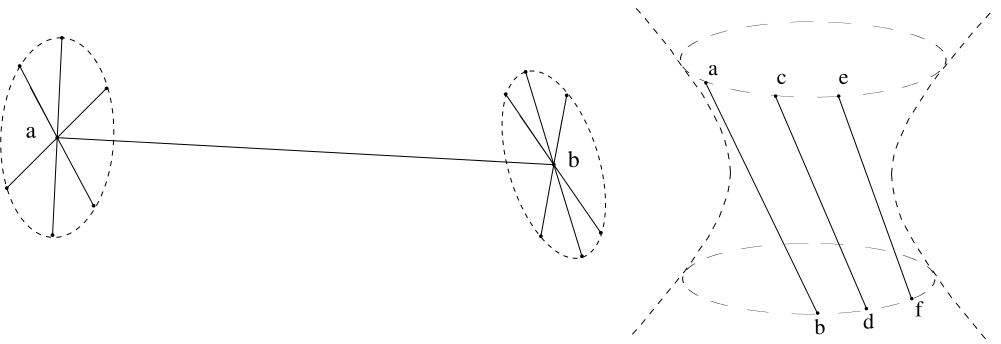
\includegraphics[width=0.6\textwidth]{subspaces2}\\
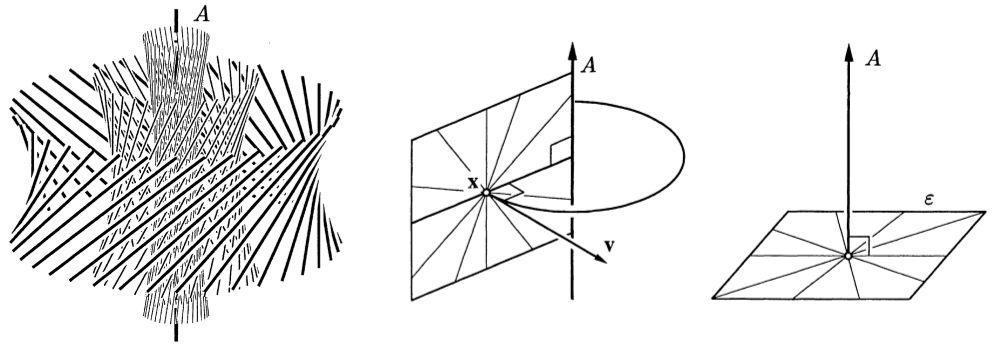
\includegraphics[width=0.6\textwidth]{subspaces1}
\end{center}
}
\end{frame}

\begin{frame}{Computing geometric interpretation}

How to recognize what to draw?
\begin{itemize}
\item Looking at basis elements is not enough
\item Intersection
\item Factorisation
\end{itemize}
\begin{figure}[b]
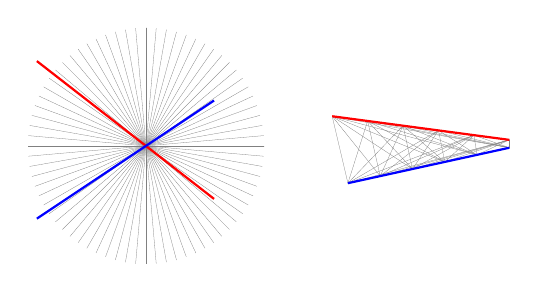
\begin{tikzpicture}
\coordinate (A1) at (-0.75, 1);
\coordinate (A2) at (1.5, -0.75);
\coordinate (B1) at (-0.75, -1);
\coordinate (B2) at (1.5, 0.5);
\coordinate (C) at (intersection cs: first line={(A1) -- (A2)}, second line={(B1)--(B2)});

\coordinate (x1) at (-0.75, 0.3);
\coordinate (x2) at (1.5, 0.0);
\coordinate (y1) at (-0.55, -0.55);
\coordinate (y2) at (1.5, -0.10);
\coordinate (D1) at ($(x1)+(3.75, 0)$);
\coordinate (D2) at ($(x2)+(3.75, 0)$);
\coordinate (E1) at ($(y1)+(3.75, 0)$);
\coordinate (E2) at ($(y2)+(3.75, 0)$);

\draw[ultra thin, gray] (C) -- +(0:1.5) -- +(0:-1.5);
\draw[ultra thin, gray] (C) -- +(5:1.5) -- +(5:-1.5);
\draw[ultra thin, gray] (C) -- +(10:1.5) -- +(10:-1.5);
\draw[ultra thin, gray] (C) -- +(15:1.5) -- +(15:-1.5);
\draw[ultra thin, gray] (C) -- +(20:1.5) -- +(20:-1.5);
\draw[ultra thin, gray] (C) -- +(25:1.5) -- +(25:-1.5);
\draw[ultra thin, gray] (C) -- +(30:1.5) -- +(30:-1.5);
\draw[ultra thin, gray] (C) -- +(35:1.5) -- +(35:-1.5);
\draw[ultra thin, gray] (C) -- +(40:1.5) -- +(40:-1.5);
\draw[ultra thin, gray] (C) -- +(45:1.5) -- +(45:-1.5);
\draw[ultra thin, gray] (C) -- +(50:1.5) -- +(50:-1.5);
\draw[ultra thin, gray] (C) -- +(55:1.5) -- +(55:-1.5);
\draw[ultra thin, gray] (C) -- +(60:1.5) -- +(60:-1.5);
\draw[ultra thin, gray] (C) -- +(65:1.5) -- +(65:-1.5);
\draw[ultra thin, gray] (C) -- +(70:1.5) -- +(70:-1.5);
\draw[ultra thin, gray] (C) -- +(75:1.5) -- +(75:-1.5);
\draw[ultra thin, gray] (C) -- +(80:1.5) -- +(80:-1.5);
\draw[ultra thin, gray] (C) -- +(85:1.5) -- +(85:-1.5);
\draw[ultra thin, gray] (C) -- +(90:1.5) -- +(90:-1.5);
\draw[ultra thin, gray] (C) -- +(95:1.5) -- +(95:-1.5);
\draw[ultra thin, gray] (C) -- +(100:1.5) -- +(100:-1.5);
\draw[ultra thin, gray] (C) -- +(105:1.5) -- +(105:-1.5);
\draw[ultra thin, gray] (C) -- +(110:1.5) -- +(110:-1.5);
\draw[ultra thin, gray] (C) -- +(115:1.5) -- +(115:-1.5);
\draw[ultra thin, gray] (C) -- +(120:1.5) -- +(120:-1.5);
\draw[ultra thin, gray] (C) -- +(125:1.5) -- +(125:-1.5);
\draw[ultra thin, gray] (C) -- +(130:1.5) -- +(130:-1.5);
\draw[ultra thin, gray] (C) -- +(135:1.5) -- +(135:-1.5);
\draw[ultra thin, gray] (C) -- +(140:1.5) -- +(140:-1.5);
\draw[ultra thin, gray] (C) -- +(145:1.5) -- +(145:-1.5);
\draw[ultra thin, gray] (C) -- +(150:1.5) -- +(150:-1.5);
\draw[ultra thin, gray] (C) -- +(155:1.5) -- +(155:-1.5);
\draw[ultra thin, gray] (C) -- +(160:1.5) -- +(160:-1.5);
\draw[ultra thin, gray] (C) -- +(165:1.5) -- +(165:-1.5);
\draw[ultra thin, gray] (C) -- +(170:1.5) -- +(170:-1.5);
\draw[ultra thin, gray] (C) -- +(175:1.5) -- +(175:-1.5);


\draw[ultra thin, gray] ($(D1)!0.0!(D2)$) -- ($(E1)!0.0!(E2)$);
\draw[ultra thin, gray] ($(D1)!0.0!(D2)$) -- ($(E1)!0.2!(E2)$);
\draw[ultra thin, gray] ($(D1)!0.0!(D2)$) -- ($(E1)!0.4!(E2)$);
\draw[ultra thin, gray] ($(D1)!0.0!(D2)$) -- ($(E1)!0.6!(E2)$);
\draw[ultra thin, gray] ($(D1)!0.0!(D2)$) -- ($(E1)!0.8!(E2)$);
\draw[ultra thin, gray] ($(D1)!0.0!(D2)$) -- ($(E1)!1.0!(E2)$);
\draw[ultra thin, gray] ($(D1)!0.2!(D2)$) -- ($(E1)!0.0!(E2)$);
\draw[ultra thin, gray] ($(D1)!0.2!(D2)$) -- ($(E1)!0.2!(E2)$);
\draw[ultra thin, gray] ($(D1)!0.2!(D2)$) -- ($(E1)!0.4!(E2)$);
\draw[ultra thin, gray] ($(D1)!0.2!(D2)$) -- ($(E1)!0.6!(E2)$);
\draw[ultra thin, gray] ($(D1)!0.2!(D2)$) -- ($(E1)!0.8!(E2)$);
\draw[ultra thin, gray] ($(D1)!0.2!(D2)$) -- ($(E1)!1.0!(E2)$);
\draw[ultra thin, gray] ($(D1)!0.4!(D2)$) -- ($(E1)!0.0!(E2)$);
\draw[ultra thin, gray] ($(D1)!0.4!(D2)$) -- ($(E1)!0.2!(E2)$);
\draw[ultra thin, gray] ($(D1)!0.4!(D2)$) -- ($(E1)!0.4!(E2)$);
\draw[ultra thin, gray] ($(D1)!0.4!(D2)$) -- ($(E1)!0.6!(E2)$);
\draw[ultra thin, gray] ($(D1)!0.4!(D2)$) -- ($(E1)!0.8!(E2)$);
\draw[ultra thin, gray] ($(D1)!0.4!(D2)$) -- ($(E1)!1.0!(E2)$);
\draw[ultra thin, gray] ($(D1)!0.6!(D2)$) -- ($(E1)!0.0!(E2)$);
\draw[ultra thin, gray] ($(D1)!0.6!(D2)$) -- ($(E1)!0.2!(E2)$);
\draw[ultra thin, gray] ($(D1)!0.6!(D2)$) -- ($(E1)!0.4!(E2)$);
\draw[ultra thin, gray] ($(D1)!0.6!(D2)$) -- ($(E1)!0.6!(E2)$);
\draw[ultra thin, gray] ($(D1)!0.6!(D2)$) -- ($(E1)!0.8!(E2)$);
\draw[ultra thin, gray] ($(D1)!0.6!(D2)$) -- ($(E1)!1.0!(E2)$);
\draw[ultra thin, gray] ($(D1)!0.8!(D2)$) -- ($(E1)!0.0!(E2)$);
\draw[ultra thin, gray] ($(D1)!0.8!(D2)$) -- ($(E1)!0.2!(E2)$);
\draw[ultra thin, gray] ($(D1)!0.8!(D2)$) -- ($(E1)!0.4!(E2)$);
\draw[ultra thin, gray] ($(D1)!0.8!(D2)$) -- ($(E1)!0.6!(E2)$);
\draw[ultra thin, gray] ($(D1)!0.8!(D2)$) -- ($(E1)!0.8!(E2)$);
\draw[ultra thin, gray] ($(D1)!0.8!(D2)$) -- ($(E1)!1.0!(E2)$);
\draw[ultra thin, gray] ($(D1)!1.0!(D2)$) -- ($(E1)!0.0!(E2)$);
\draw[ultra thin, gray] ($(D1)!1.0!(D2)$) -- ($(E1)!0.2!(E2)$);
\draw[ultra thin, gray] ($(D1)!1.0!(D2)$) -- ($(E1)!0.4!(E2)$);
\draw[ultra thin, gray] ($(D1)!1.0!(D2)$) -- ($(E1)!0.6!(E2)$);
\draw[ultra thin, gray] ($(D1)!1.0!(D2)$) -- ($(E1)!0.8!(E2)$);
\draw[ultra thin, gray] ($(D1)!1.0!(D2)$) -- ($(E1)!1.0!(E2)$);

\draw[thick, red] (A1) -- (A2);
\draw[thick, blue] (B1) -- (B2);

\draw[thick, red] (D1) -- (D2);
\draw[thick, blue] (E1) -- (E2);
\end{tikzpicture}
\end{figure}
\end{frame}

\begin{frame}{Implement drawing routines}
\only<1>{
GAViewer
\begin{itemize}
\item Graphing calculator for geometric algebra
\item Models for Euclidean and conformal geometric algebra
\end{itemize}
\begin{center}
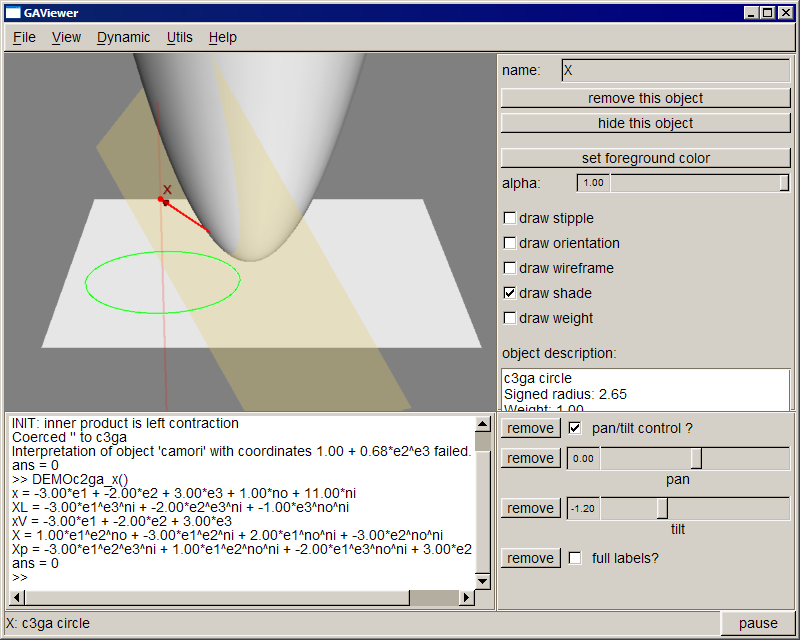
\includegraphics[width=0.6\textwidth]{gaviewer}
\end{center}
}

\only<2>{
Interface challenges
\begin{itemize}
\item Line density
\item Objects at infinity
\item Translation-invariant objects
\item Rotation-invariant objects
\item User interaction
\end{itemize}
}
\end{frame}

\begin{frame}
\begin{center}
{\Large\structure{Questions}}
\end{center}
\end{frame}
\end{document}
